\documentclass[a4paper, 12pt]{article}
\usepackage[usenames,dvipsnames,svgnames,table]{xcolor}
\usepackage[T1]{fontenc}
\usepackage{float}
\usepackage{times}
\usepackage[utf8]{inputenc}
\usepackage{wallpaper}
\usepackage[absolute]{textpos}
\usepackage[top=2cm, bottom=2.5cm, left=3cm, right=3cm]{geometry}

\newsavebox{\mybox}
\newlength{\mydepth}
\newlength{\myheight}
\newenvironment{sidebar}
{\begin{lrbox}{\mybox}\begin{minipage}{\textwidth}}
{\end{minipage}\end{lrbox}
 \settodepth{\mydepth}{\usebox{\mybox}}
 \settoheight{\myheight}{\usebox{\mybox}}
 \addtolength{\myheight}{\mydepth}
 \noindent\makebox[0pt]{\hspace{-20pt}\rule[-\mydepth]{1pt}{\myheight}}
 \usebox{\mybox}}

\newcommand\BackgroundPic{
    \put(-2,-3){
    
\includegraphics[keepaspectratio,scale=0.3]{../lnu_etch.png} 
    }
}
\newcommand\BackgroundPicLogo{
    \put(30,740){
	
\includegraphics[keepaspectratio,scale=0.10]{../logo.png}     
    }
}

\title{	
\vspace{-8cm}
\begin{sidebar}
    \vspace{5cm}
    \normalfont \normalsize
    \Huge Report \\
    \vspace{-1.3cm}
\end{sidebar}
\vspace{3cm}
\begin{flushleft}
    \huge Test Cases\\  
\end{flushleft}
\null
\vfill
\begin{textblock}{6}(10,13)
\begin{flushright}
\begin{minipage}{\textwidth}
\begin{flushleft} \large
	\emph{Author:} \\ Caroline Nilsson \textit{(cn222nd)} \\ Daniel Alm Grundström \textit{(dg222dw)} \\
	%\emph{Handledare:} \\ 
	\emph{Term:} HT 2017\\ 
	\emph{Course:} 2DV610 - Software Testing\\
\end{flushleft}
\end{minipage}
\end{flushright}
\end{textblock}
}
\date{\today} 

\begin{document}

\pagenumbering{gobble}
\newgeometry{left=5cm}
\AddToShipoutPicture*{\BackgroundPic}
\AddToShipoutPicture*{\BackgroundPicLogo}
\maketitle
\restoregeometry
\clearpage

\pagenumbering{gobble}

\tableofcontents
\newpage
\pagenumbering{arabic}

\newpage

\section{Use Case: Start Server}
This section provides Test Cases for Use Case 1 starting the server. Below is a list of steps that shall be performed before each Test Case.

\begin{itemize}
\item Open the terminal
\item Navigate to the .jar file location
\end{itemize}

\subsection{Unavailable socket (Manual)}

The system shall notify the administrator if the provided port socket is unavailable.\\
\textbf{Test Input} \\ Port socket: 80 \textit{incorrect} \\ Shared resource: MyWebServer-master\ 12.15.02/tests/se/lnu/http/resources/inner/ \\ \textit{correct}
 
\subsubsection{Input}
\begin{itemize}
\item input \texttt{"java -jar MyWebServer.jar \\
80 MyWebServer-master\ 12.15.02/tests/\\se/lnu/http/resources/inner/"}
\item Press enter
\item Open a web browser
\item Enter \texttt{"localhost:80"}
\item Press enter
\end{itemize} 

\subsubsection{Output}
\textbf{Web Browser}
\begin{itemize}
\item Display unable to connect to the server
\end{itemize}

\textbf{Console}
\begin{itemize}
\item \texttt{"Socket 80 was taken"} shows in console window
\end{itemize}

\subsection{Restriction on shared resource container (Manual)}

The system shall give an error when the shared resource container is protected.\\
\textbf{Test Input} \\ Port socket: 8080 \textit{correct} \\ Shared resource: \texttt{/var/root/} (MAC) \texttt{/root/} (Linux) \\ \textit{incorrect}
 
\subsubsection{Input}
\begin{itemize}
\item input \texttt{"java -jar MyWebServer.jar 8080 /root/ on Linux or /var/root on Mac"}
\item Press enter
\end{itemize} 

\subsubsection{Output}
\textbf{Console}
\begin{itemize}
\item \texttt{"No access to folder /var/root"} on Mac and \texttt{"No access to folder /root/"} on Linux shows in console window
\end{itemize}

\subsection{Access log could not be written (Manual)}

The system shall report when the access log could not be written to.\\
\textbf{Test Input} \\ Port socket: 8080 \textit{correct} \\ Shared resource: MyWebServer-master\ 12.15.02/tests/se/lnu/http/resources/inner/ \\ \textit{correct}
 
\subsubsection{Input}
\begin{itemize}
\item If there is an existing log.txt, remove it
\item Enter \texttt{"touch log.txt"}
\item Enter \texttt{"chflags uchg log.txt"} on Mac and \texttt{"chmod 000 log.txt"} on Linux
\item input \texttt{"java -jar MyWebServer.jar \\ 8080 MyWebServer-master\ 12.15.02/tests/\\se/lnu/http/resources/inner/"}
\item Press enter
\end{itemize} 

\subsubsection{Output}
\textbf{Console}
\begin{itemize}
\item \texttt{"Cannot write to server log file log.txt"} shows in console window
\end{itemize}

\subsubsection{After test}
\begin{itemize}
\item Remove log.txt \texttt{"chflags nouchg log.txt \&\& rm -f log.txt"} on Mac and \texttt{"rm -f log.txt"} on Linux
\end{itemize}

\subsection{Starting Server (Manual)}

An administrator should be able to start the server by running the .jar file and provide port socket and shared resources folder.\\
\textbf{Test Input} \\ Port socket: 8080 \\ Shared resource: MyWebServer-master\ 12.15.02/tests/se/lnu/http/resources/inner/
\subsubsection{Input}
\begin{itemize}
\item input \texttt{"java -jar MyWebServer.jar \\
8080 MyWebServer-master\ 12.15.02/tests/\\se/lnu/http/resources/inner/"}
\item Press enter key
\item Open a web browser
\item Enter \texttt{"localhost:8080"}
\item Press enter
\end{itemize}

\subsubsection{Output}
\textbf{Web Browser}
\begin{itemize}
\item "It works" is shown on the page \textit{(see figure: \ref{TC1.1})}
\end{itemize}

\textbf{Console}
\begin{itemize}
\item \texttt{"HTTP Server Started"} is shown in console window
\end{itemize}

\begin{figure}[H]
\centering
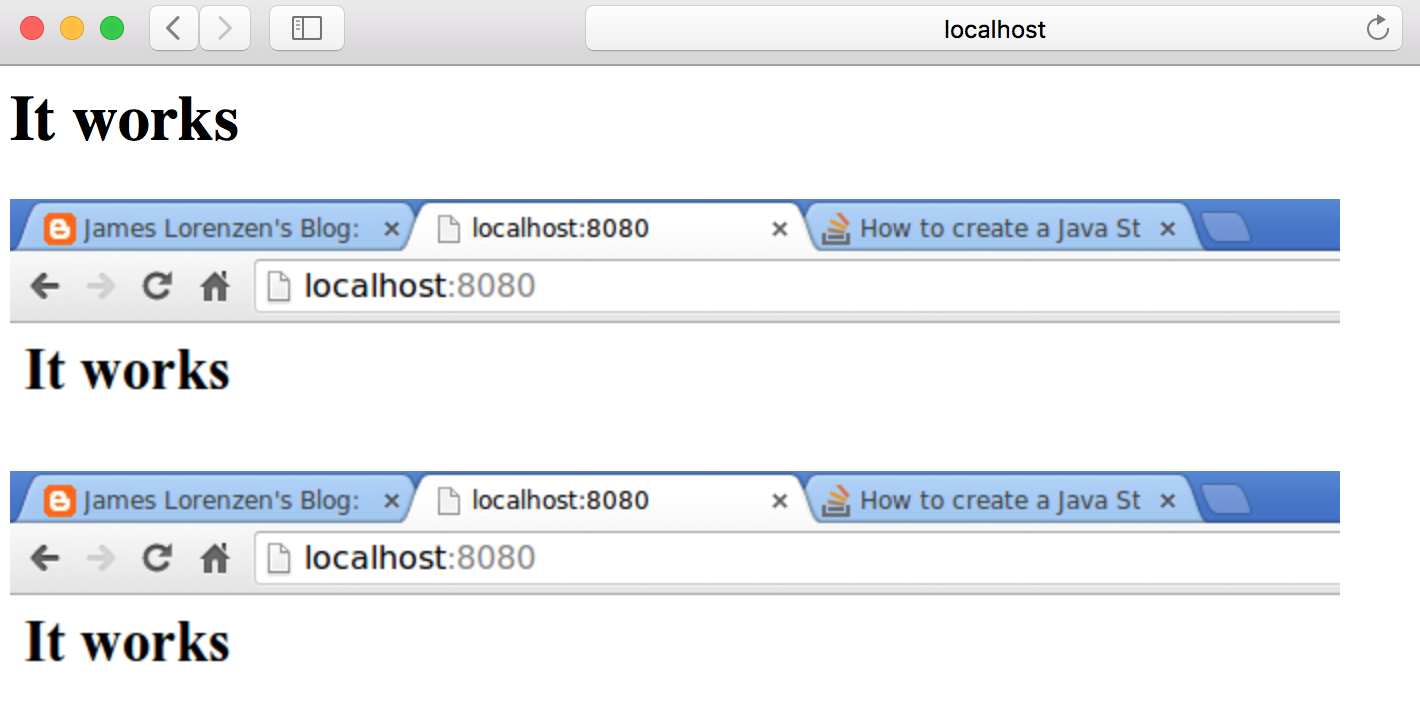
\includegraphics[scale=0.5]{output_clarification/TC1-1.png} 
\caption{Output for successfully starting server}
\label{TC1.1}
\end{figure}

\newpage
\section{Use Case: Stop Server}

Before each test in this section perform test case 1.4 in order to start the server and assure it runs correctly.

\subsection{Stopping Server (Manual)}

An administrator should be able to stop the server by inputting "stop" into a running server's command line.

\subsubsection{Input}
\begin{itemize}
\item Input "stop" into the server's command line window and press Enter
\item Open a web browser and navigate to "http://localhost:8080/"
\end{itemize}

\subsubsection{Output}
\begin{itemize}
\item A page with the header "Unable to connect" should appear in the web browser.
\end{itemize}


\subsection{Access log written to when server is stopped (Manual)}

Make sure that an entry is written to the server's access log when an administrator manually stops the server.

\subsubsection{Input}
\begin{itemize}
\item Input "stop" into server's command line window and press Enter
\item Open server access log in a text editor
\end{itemize}

\subsubsection{Output}
\begin{itemize}
\item The text "HTTP Server stopped" should be displayed on the last line of the access log.
\end{itemize}


\newpage
\section{Use Case: Request Shared Resource}

Before each test in this section perform test case 1.4 in order to start the server and assure it runs correctly.

\subsection{Return Response 200 OK (JMeter)}

Ensure that the server return HTTP 1.1 response 200 when a request was successful.

\subsubsection{Input}
\begin{itemize}
\item \textit{HTTP Request} GET: \texttt{"index.html"}
\item Run test
\end{itemize}

\subsubsection{Output}
\begin{itemize}
\item Server response with response code 200 \textit{(See fig. \ref{TC3.1})}
\end{itemize}

\begin{figure}[H]
\centering
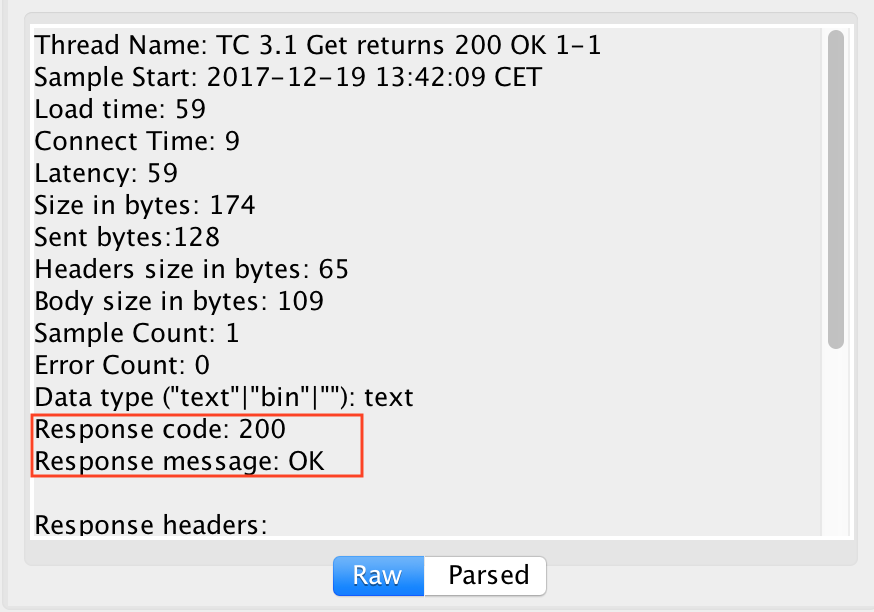
\includegraphics[scale=0.7]{output_clarification/200OK.png} 
\caption{200 OK}
\label{TC3.1}
\end{figure}


\subsection{Return Response 404 NOT FOUND (JMeter)}

Ensure that the server return HTTP 1.1 response 404 when a requested resource does not exist.

\subsubsection{Input}
\begin{itemize}
\item \textit{HTTP Request} GET: \texttt{"nonexistingfile.txt"}
\item Run test
\end{itemize}

\subsubsection{Output}
\begin{itemize}
\item Server response with response code 404 \textit{(See fig. \ref{TC3.2})}
\end{itemize}

\begin{figure}[H]
\centering
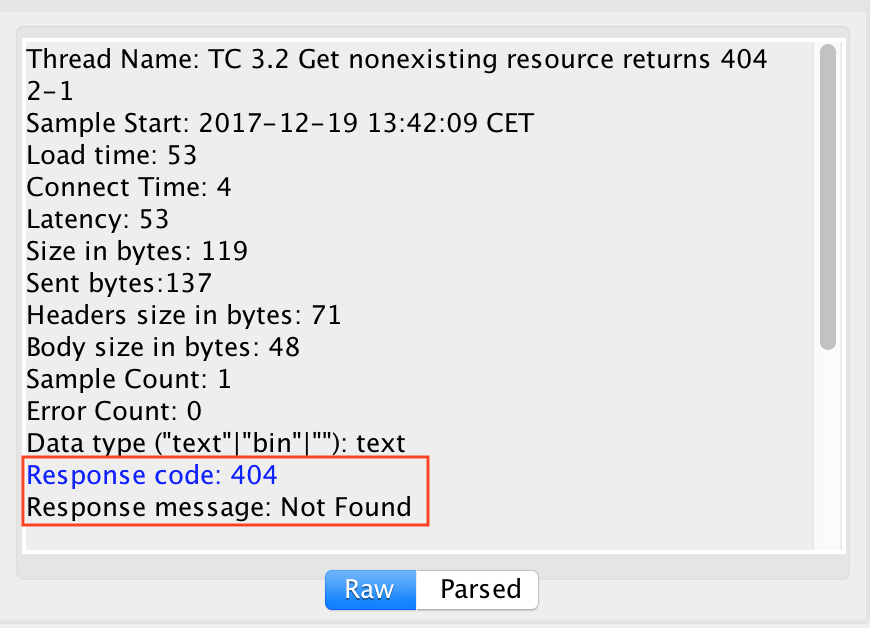
\includegraphics[scale=0.7]{output_clarification/404NOTFOUND.png} 
\caption{404 Not Found}
\label{TC3.2}
\end{figure}


\subsection{Return Response 403 FORBIDDEN (JMeter)}

Ensure that the server return HTTP 1.1 response 403 when the requested resource is outside the shared resource container.

\subsubsection{Input}
\begin{itemize}
\item \textit{HTTP Request} GET: \texttt{"../secret.html"}
\item Run test
\end{itemize}

\subsubsection{Output}
\begin{itemize}
\item Server response with response code 403 \textit{(See fig. \ref{TC3.3})}
\end{itemize}

\begin{figure}[H]
\centering
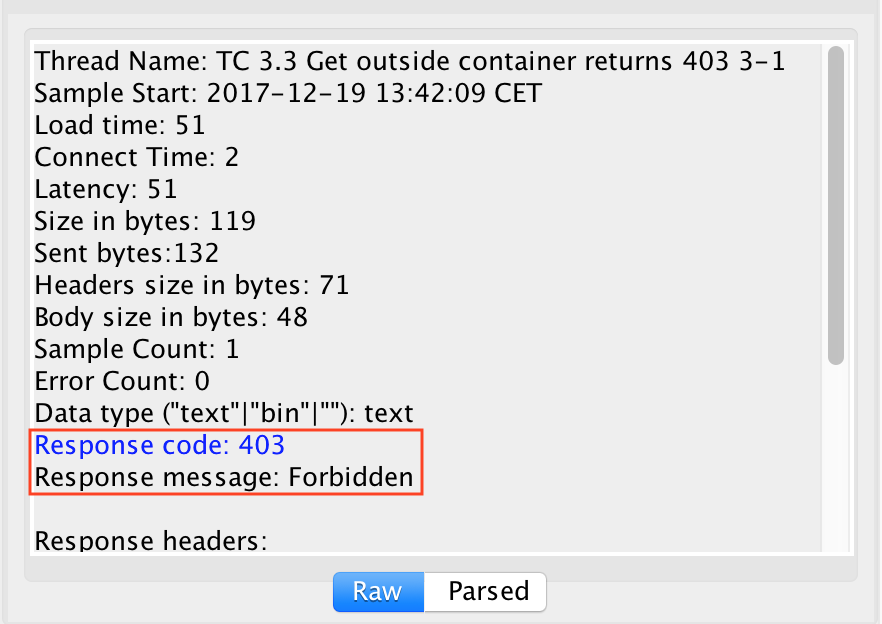
\includegraphics[scale=0.7]{output_clarification/403FORBIDDEN.png} 
\caption{403 Forbidden}
\label{TC3.3}
\end{figure}

\subsection{Return Response 400 BAD REQUEST (JMeter)}

Ensure that the server return HTTP 1.1 response 400 when the URL is malformed.

\subsubsection{Input}
\begin{itemize}
\item \textit{HTTP Request} GET: \texttt{"\%index.html"}
\item Run test
\end{itemize}

\subsubsection{Output}
\begin{itemize}
\item Server response with response code 400 \textit{(See fig. \ref{TC3.4})}
\end{itemize}

\begin{figure}[H]
\centering
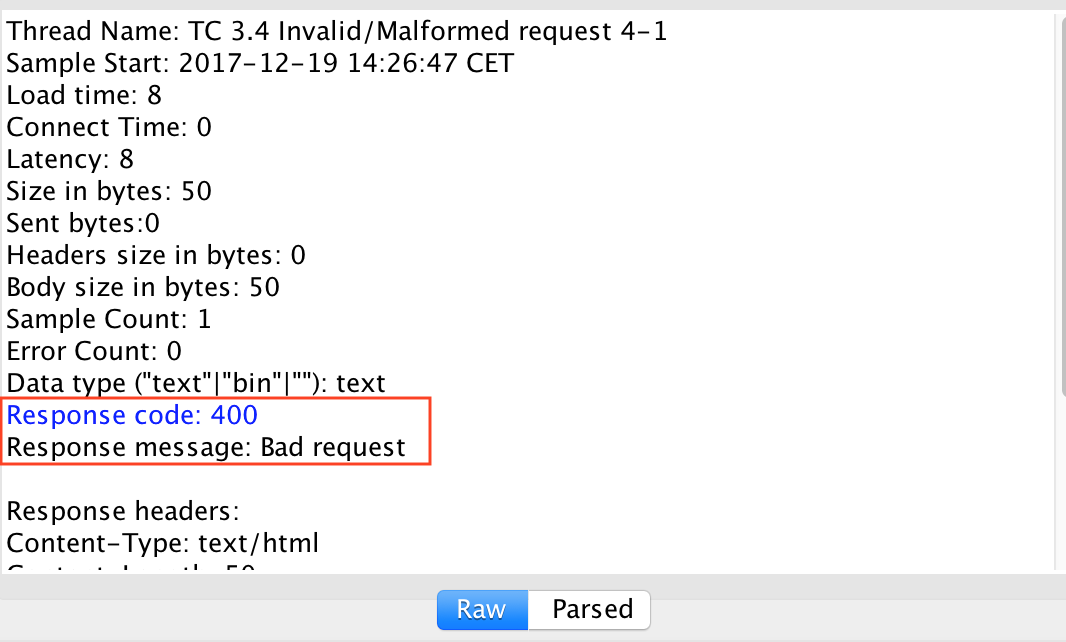
\includegraphics[scale=0.7]{output_clarification/400BADREQUEST.png} 
\caption{Bad Request}
\label{TC3.4}
\end{figure}

\newpage
\section{Requirement: 1 Responsive Under High Load}

\subsection{System response time (JMeter)}

The system should response within 2 seconds when no more than 100 users access the shared resources.

\subsubsection{Input}
\begin{itemize}
\item Perform test case 1.4
\item \textit{Thread Group} Users: 100
\item \textit{Thread Group} Loop Count: 1000
\item \textit{HTTP Request} GET: \texttt{"index.html"}
\item Run test
\end{itemize}

\subsubsection{Output}
\begin{itemize}
\item maximum server response time does not exceed 2000 ms (2 sec) \textit{(See fig. \ref{TC4.1})}
\end{itemize}

\begin{figure}[H]
\centering
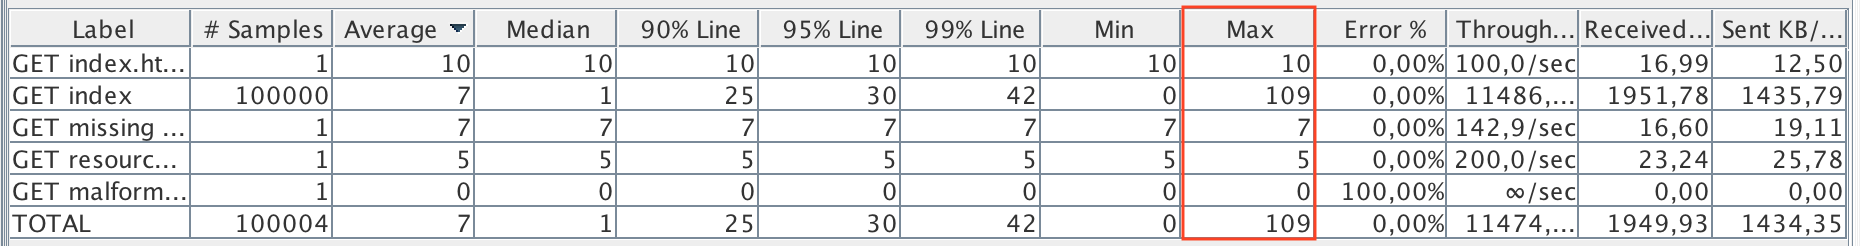
\includegraphics[scale=0.5]{output_clarification/HighLoad.png} 
\caption{Maximum Server Response Time}
\label{TC4.1}
\end{figure}

\newpage

\section{Requirement: 5 Access Log}

Before each test in this section perform test case 1.4 in order to start the server and assure it runs correctly.

\subsection{Get Picture (Manual)}

When a user has accessed a picture from the web servers shared resource container it should be stated in the access log.

\subsubsection{Input}
\begin{itemize}
\item Open a web browser
\item Input \texttt{"localhost:8080/images/works.png"} into the address bar
\item Press enter
\item \textit{The picture should be shown in the web browser}
\item Naviagate to the log.txt location and open the access log
\end{itemize}


\subsubsection{Output}
\begin{itemize}
\item \texttt{"Clientthread \# served file : works.png"} should be printed in the log file \textit{(\# represents the thread number)}
\end{itemize}

\newpage
\section{Informal Requirement: Usability}

\subsection{Faulty Parameter (Manual)}

The web server should show help text informing the user on how to start the server when the user gives a faulty command line argument. 

\subsubsection{Input}
\begin{itemize}
\item Navigate to the MyWebServer.jar folder in the console window
\item Input \texttt{"java -jar MyWebServer.jar 0"}
\item Press enter
\end{itemize} 

\subsubsection{Output} 
\begin{itemize}
\item The text \texttt{"Enter a valid port 1-65 535 and a optional URL"} is shown in the console window
\end{itemize}

\subsection{--help Command (Manual)}

A help section with information about the web server and how to use it should be shown when the input \texttt{--help} is given as parameter.

\subsubsection{Input}
\begin{itemize}
\item Navigate to the MyWebServer.jar folder in the console window
\item Input \texttt{"java -jar MyWebServer.jar --help"}
\item Press enter
\end{itemize} 

\subsubsection{Output}
\textbf{Text that shall be shown in console window}
\begin{itemize}
\item \texttt{MyWebServer}
\item \texttt{To start the server enter java -jar MyWebServer.jar <Port> <Shared Resource>}
\item \texttt{The Port need to be 1-65 535 and unused}
\item \texttt{The user who starts the server needs to have read-access to the shared resource}
\item \texttt{Licence: GPL-2.0}
\item \texttt{2017 Software Development Company (SDC)}
\end{itemize}

\newpage
\section{Informal Requirement: Security}

Before each test in this section perform test case 1.4 in order to start the server and assure it runs correctly.

\subsection{HTTPS (Manual)}

The web server shall use \textit{HTTPS} as standard.

\subsubsection{Input}
\begin{itemize}
\item Open a web browser
\item Enter \texttt{"https://localhost:8080"} into the address bar
\item Press enter
\end{itemize}

\subsubsection{Output}
\begin{itemize}
\item "It works" is shown on the page \textit{(see figure: \ref{TC6.1})}
\end{itemize}

\begin{figure}[H]
\centering
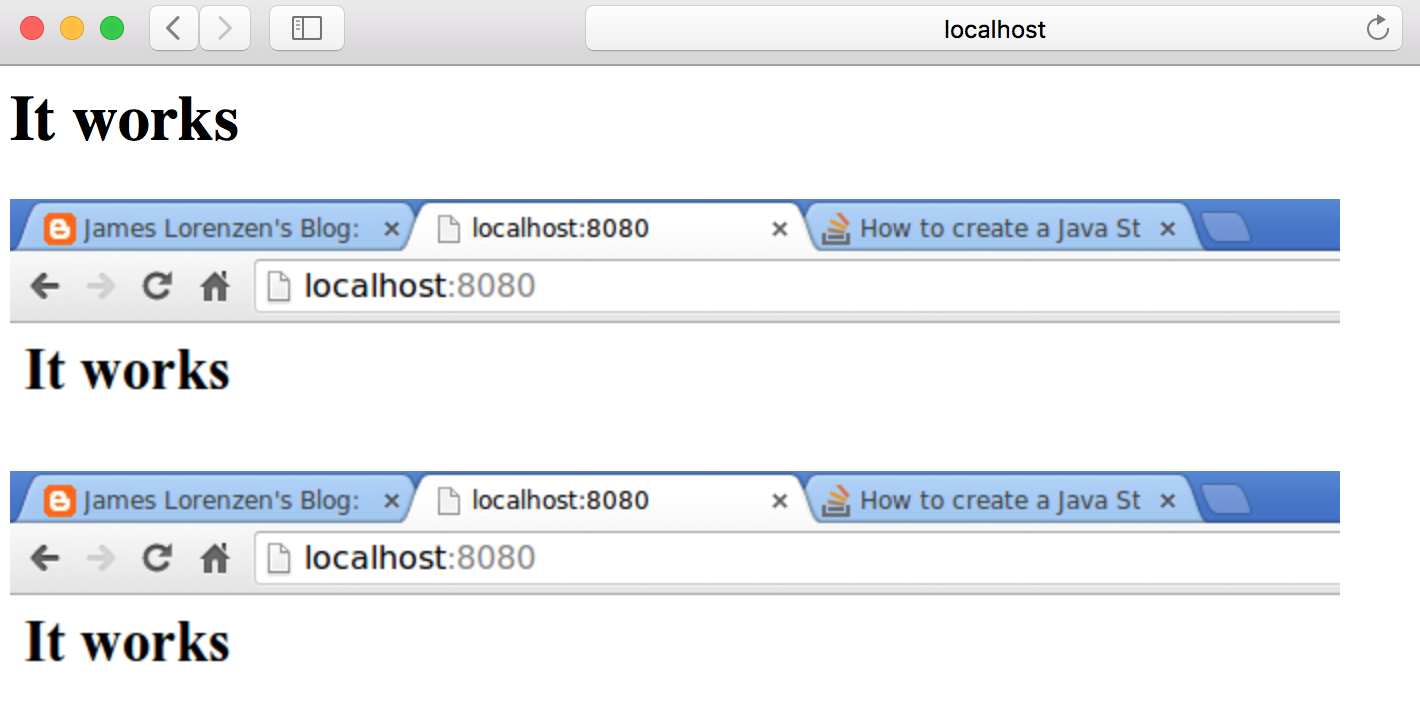
\includegraphics[scale=0.5]{output_clarification/TC1-1.png} 
\caption{Output for successfully starting server}
\label{TC6.1}
\end{figure}

\subsection{Trace (JMeter)}

The web server shall have Trace disabled to prevent \textit{Cross Site Tracing} attacks.

\subsubsection{Input}
\begin{itemize}
\item \textit{HTTP Request} TRACE:
\item Run test
\end{itemize}

\subsubsection{Output}
\begin{itemize}
\item Server response with response code 405 \textit{(See fig. \ref{TC7.1})}
\end{itemize}

\begin{figure}[H]
\centering
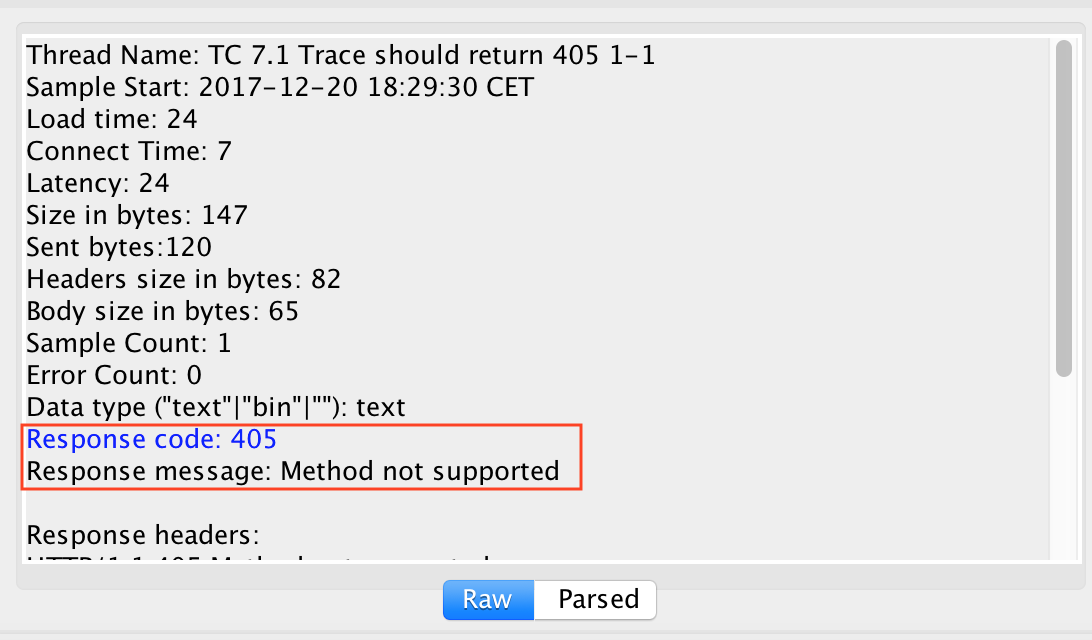
\includegraphics[scale=0.7]{output_clarification/405METHODNOTSUPORTED.png} 
\caption{405 Method Not Supported}
\label{TC7.1}
\end{figure}

\end{document}


